\subsection*{Experiment 8.15 \quad Measurement of the wavelength of laser light}

\textbf{[Apparatus and materials available]} One semiconductor laser, tape measure, steel ruler (with 0.5 mm graduations), retort stand, optical bench, white paper screen.

\textbf{[Requirements]}

(1) Briefly describe the experimental steps and derive the formula.

(2) Record the experimental data and calculate the wavelength of the laser light.

Note: when a laser beam is incident obliquely on the graduations of a steel ruler, diffraction occurs. Let the angle between the incident laser beam and the surface of the steel ruler be $\theta_0$, and the angle between the diffracted ray of order $K$ and the steel ruler be $\theta_K$; then the diffraction spots satisfy the relation
\[
d(\cos\theta_0-\cos\theta_K)=K\lambda,
\]
where $\lambda$ is the laser wavelength and $d$ the grating constant, that is, the distance between adjacent graduations of the steel ruler.

\textbf{Solution 8.15}\quad \textbf{1.} A laser beam is directed at the end of the steel ruler. Part of the light passes directly above the ruler and falls on the observation screen at the point $-S_0$; the rest is reflected from the surface of the ruler onto the screen. Besides the reflected bright spot at $S_0$, which is symmetric to $-S_0$, a whole series of bright spots $S_1$, $S_2$, $S_3$, $S_4$, $\ldots$ can be seen on the screen. This is because the ruler bears scratches (the spacing of the scratches is $d=0.5\,\mathrm{mm}$). Light is reflected from the many smooth surfaces between two scratches. If these reflected beams have the same phase (that is, crest meets crest and trough meets trough), they superpose and reinforce each other, forming a bright spot; otherwise they cancel and the light is weakened. As shown in Fig.~1, the laser beam is incident on the end face of the steel ruler, and the reflected light forms the diffraction pattern.

\begin{figbox}{8.15(a)}
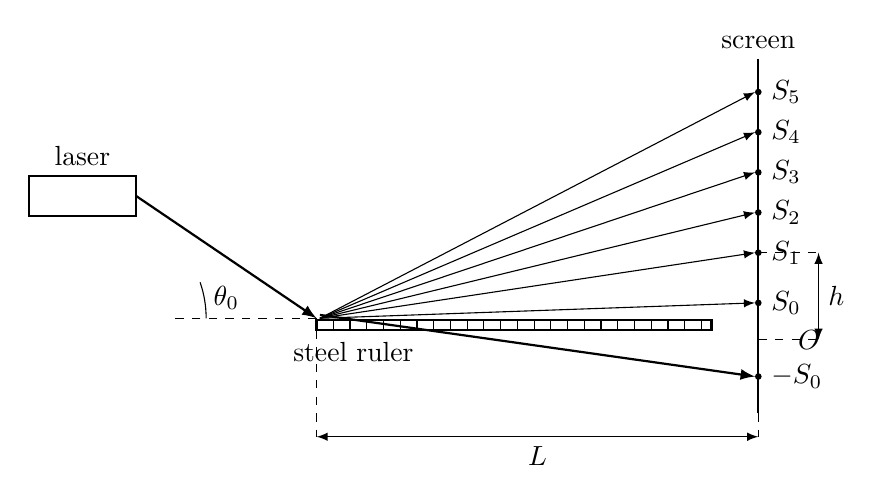
\begin{tikzpicture}[x=0.85cm,y=0.85cm,>=latex]
% screen
\draw[thick] (6.6,-1.4) -- (6.6,3.9);
\node[above] at (6.6,3.9) {screen};
% ruler
\draw[thick] (0,0) -- (5.9,0) -- (5.9,-0.16) -- (0,-0.16) -- cycle;
\foreach \x in {0.25,0.5,...,5.75} \draw (\x,0) -- (\x,-0.16);
\node[below] at (0.55,-0.2) {steel ruler};
% laser
\draw[thick] (-4.3,1.55) rectangle (-2.7,2.15);
\node[above] at (-3.5,2.15) {laser};
% incident beam
\draw[->,thick] (-2.7,1.85) -- (0,0.02);
% angle theta0 between beam and ruler surface
\draw[dashed] (0,0.02) -- (-2.2,0.02);
\draw (-1.65,0.02) arc (0:19:1.65);
\node at (-1.35,0.32) {$\theta_0$};
% reflected fan
\foreach \y/\lab in {0.25/{$S_0$},1.0/{$S_1$},1.6/{$S_2$},2.2/{$S_3$},2.8/{$S_4$},3.4/{$S_5$}}{
  \draw[->] (0.05,0.02) -- (6.55,\y);
  \fill (6.6,\y) circle (1.2pt);
  \node[right] at (6.65,\y) {\lab};
}
% direct beam to -S0
\draw[->,thick] (0.05,0.07) -- (6.55,-0.85);
\fill (6.6,-0.85) circle (1.2pt);
\node[right] at (6.65,-0.85) {$-S_0$};
\node[right] at (7.05,-0.3) {$O$};
% h dimension
\draw[<->] (7.5,-0.3) -- (7.5,1.0) node[midway,right] {$h$};
\draw[dashed] (6.6,-0.3) -- (7.5,-0.3);
\draw[dashed] (6.6,1.0) -- (7.5,1.0);
% L dimension
\draw[<->] (0,-1.75) -- (6.6,-1.75) node[midway,below] {$L$};
\draw[dashed] (0,-0.16) -- (0,-1.75);
\draw[dashed] (6.6,-1.4) -- (6.6,-1.75);
\end{tikzpicture}
\end{figbox}

From Fig.~2 it can be seen that the path difference (called the optical path difference) accumulated by light emitted from a point $A$ of the source and reflected at two adjacent smooth surfaces $B$ and $B'$ in reaching the point $C$ on the screen is
\begin{equation}
\Delta=AB'C-ABC=DB'-BD'=d(\cos\alpha-\cos\beta) \tag{1}
\end{equation}

\begin{figbox}{8.15(b)}
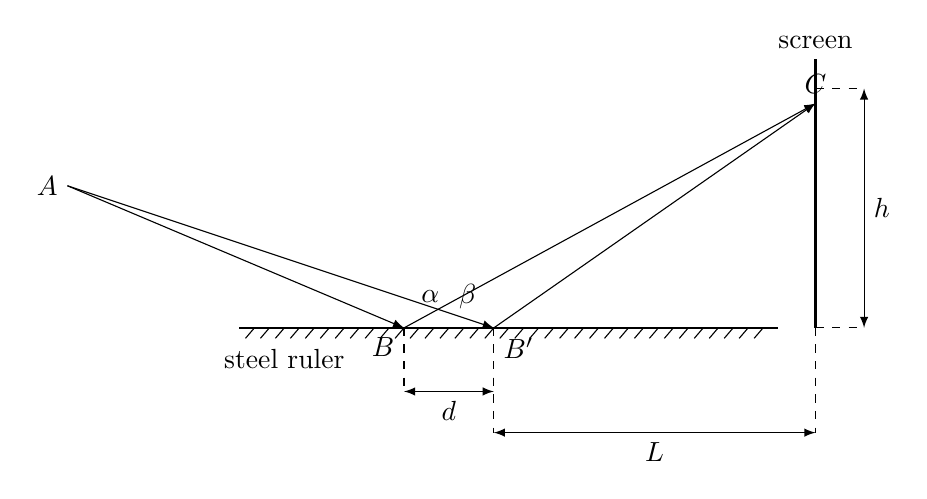
\begin{tikzpicture}[x=0.95cm,y=0.95cm,>=latex]
% screen
\draw[thick] (7.7,0) -- (7.7,3.6);
\node[above] at (7.7,3.6) {screen};
% ruler
\draw[thick] (0,0) -- (7.2,0);
\foreach \x in {0.2,0.4,...,7.0} \draw (\x,0) -- (\x-0.12,-0.14);
\node[below] at (0.6,-0.15) {steel ruler};
% points
\coordinate (A) at (-2.3,1.9);
\coordinate (B) at (2.2,0);
\coordinate (Bp) at (3.4,0);
\coordinate (C) at (7.7,3.0);
% rays
\draw[->] (A) -- (B);
\draw[->] (A) -- (Bp);
\draw[->] (B) -- (C);
\draw[->] (Bp) -- (C);
\node[left] at (A) {$A$};
\node[below left] at (B) {$B$};
\node[below right] at (Bp) {$B'$};
\node[above] at (C) {$C$};
% angle labels
\node at (2.55,0.42) {$\alpha$};
\node at (3.05,0.42) {$\beta$};
% d dimension
\draw[<->] (2.2,-0.85) -- (3.4,-0.85) node[midway,below] {$d$};
\draw[dashed] (2.2,0) -- (2.2,-0.85);
\draw[dashed] (3.4,0) -- (3.4,-0.85);
% L and h
\draw[<->] (3.4,-1.4) -- (7.7,-1.4) node[midway,below] {$L$};
\draw[dashed] (3.4,0) -- (3.4,-1.4);
\draw[dashed] (7.7,0) -- (7.7,-1.4);
\draw[<->] (8.35,0) -- (8.35,3.2) node[midway,right] {$h$};
\draw[dashed] (7.7,0) -- (8.35,0);
\draw[dashed] (7.7,3.2) -- (8.35,3.2);
\end{tikzpicture}
\end{figbox}

If $\Delta$ happens to be zero or an integral multiple of the wavelength $\lambda$, the phases of these reflected beams are the same, and a bright spot appears at the point $C$ on the screen. Obviously, at $\beta=\alpha$ one has $\Delta=0$, and this is the bright spot at $S_0$. At $S_1$, $S_2$, $S_3$, $S_4$, $\ldots$ one must have $\Delta_1=\lambda$, $\Delta_2=2\lambda$, $\Delta_3=3\lambda$, $\Delta_4=4\lambda$, $\ldots$; hence from (1) it follows that
\begin{align}
d(\cos\alpha-\cos\beta_1)&=\lambda, \tag{2}\\
d(\cos\alpha-\cos\beta_2)&=2\lambda, \tag{3}\\
d(\cos\alpha-\cos\beta_3)&=3\lambda, \tag{4}\\
d(\cos\alpha-\cos\beta_4)&=4\lambda. \tag{5}
\end{align}
Here $d=0.500\,\mathrm{mm}$ is known. Therefore, provided that $\alpha$ and $\beta_1$, $\beta_2$, $\beta_3$, $\beta_4$, $\ldots$ are measured, the wavelength $\lambda$ can be calculated from each of these equations. In the experiment the ruler is set perpendicular to the screen, so that
\begin{equation}
\tan\beta=h/L. \tag{6}
\end{equation}
Here $L$ is the distance from the end of the ruler to the screen, and $h$ is the distance from each bright spot to the point $O$, where $O$ lies midway between $S_0$ and $-S_0$. By measuring the distances of the bright spots one obtains the values of $\beta_k$; for the bright spot $S_0$ the angle $\beta$ is just $\alpha$.

\textbf{2. Experimental steps}

(1) Place the steel ruler on the optical bench in a horizontal position. Fix the laser on a retort stand and let the semiconductor laser beam fall on the end face of the steel ruler at an angle of $2\degree$ to the surface of the bench. Place the white screen at a distance of about $2\,\mathrm{m}$ from the steel ruler, with the ruler perpendicular to the screen. (A wall may be used instead of the screen.)

(2) Paste a strip of white paper on the screen (or wall) and mark on it the positions of the bright spots $-S_0$, $S_0$, $S_1$, $S_2$, $S_3$, $S_4$, etc. (Take care to identify the position of $S_0$ correctly and never mistake it; the position of $S_0$ can be identified by allowing the laser to fall on a part of the steel ruler that bears no scratches.)

3. Use the tape measure to find the distance $L$ from the front end of the steel ruler to the wall.

4. Take the paper strip down from the wall and take the midpoint of $-S_0$ and $S_0$ as the point $O$. Measure the distances of the points $S_0$, $S_1$, $S_2$, $S_3$, $S_4$, $\ldots$ from $O$ (these are the values of $h$), calculate $\alpha$ and $\beta$ from (6) (the $\beta$ corresponding to $S_0$ is $\alpha$), and then calculate $\lambda$ from each of equations (2)--(5); take the average as the wavelength of the semiconductor laser.

\begin{commentary}
In this experiment the graduations of a steel ruler serve as a ``grating'', so the experiment belongs to the class of ``reflection grating'' diffraction experiments.
\end{commentary}

\subsection*{Experiment 8.16 \quad Making a double slit, measuring its interference fringes and finding the slit separation $d$}

\textbf{[Apparatus and materials available]} One helium--neon laser ($\lambda=633\,\mathrm{nm}$), light screen, support, tape measure, coordinate paper, card paper, two double-edged razor blades.

\textbf{[Requirements]}

(1) Make a suitable double slit and write down the procedure.

(2) Draw the arrangement of the apparatus and the ray diagram, and write down the relevant formulas.

(3) Perform the experiment and find the separation $d$ of the two slits.

\textbf{Solution 8.16}\quad \textbf{1.} Place the two razor blades together with one or two sheets of paper between them, and draw them lightly once across the card paper supplied, so as to make a double slit of width $d$ of about $0.3$--$0.5\,\mathrm{mm}$.

2. The experimental arrangement is shown in Fig.~1.

\begin{figbox}{8.16(a)}
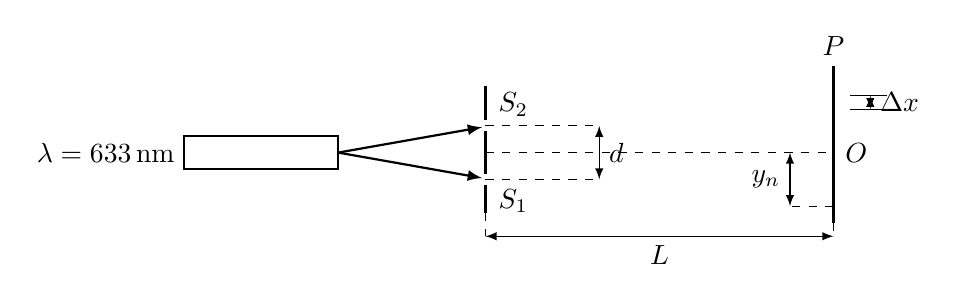
\begin{tikzpicture}[x=0.85cm,y=0.85cm,>=latex]
% laser
\draw[thick] (0,0.85) rectangle (2.3,1.35);
\node[left] at (0,1.1) {$\lambda=633\,\mathrm{nm}$};
% beam
\draw[->,thick] (2.3,1.1) -- (4.45,0.72);
\draw[->,thick] (2.3,1.1) -- (4.45,1.48);
% slit plane with two gaps
\draw[thick] (4.5,0.2) -- (4.5,0.62);
\draw[thick] (4.5,0.78) -- (4.5,1.42);
\draw[thick] (4.5,1.58) -- (4.5,2.1);
\node[below right] at (4.55,0.70) {$S_1$};
\node[above right] at (4.55,1.50) {$S_2$};
% d dimension
\draw[<->] (6.2,0.70) -- (6.2,1.50) node[midway,right] {$d$};
\draw[dashed] (4.5,0.70) -- (6.2,0.70);
\draw[dashed] (4.5,1.50) -- (6.2,1.50);
% screen
\draw[thick] (9.7,0.05) -- (9.7,2.4);
\node[above] at (9.7,2.4) {$P$};
% axis
\draw[dashed] (4.5,1.1) -- (9.7,1.1);
\node[right] at (9.73,1.1) {$O$};
% y_n dimension
\draw[<->] (9.05,1.1) -- (9.05,0.3) node[midway,left] {$y_n$};
\draw[dashed] (9.7,0.3) -- (9.05,0.3);
% fringe spacing at the top of the screen
\draw (9.95,1.95) -- (10.5,1.95);
\draw (9.95,1.75) -- (10.5,1.75);
\draw[<->] (10.25,1.75) -- (10.25,1.95) node[midway,right] {$\Delta x$};
% L dimension
\draw[<->] (4.5,-0.15) -- (9.7,-0.15) node[midway,below] {$L$};
\draw[dashed] (4.5,0.2) -- (4.5,-0.15);
\draw[dashed] (9.7,0.05) -- (9.7,-0.15);
\end{tikzpicture}
\end{figbox}

\begin{figbox}{8.16(b)}
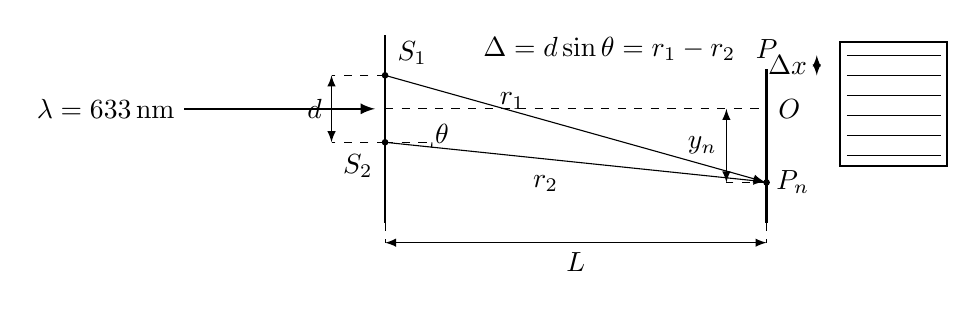
\begin{tikzpicture}[x=0.85cm,y=0.85cm,>=latex]
% slit plane and screen
\draw[thick] (3.2,0.2) -- (3.2,3.0);
\draw[thick] (8.9,0.2) -- (8.9,2.5);
\node[above] at (8.9,2.5) {$P$};
% slits
\fill (3.2,2.4) circle (1.2pt);
\fill (3.2,1.4) circle (1.2pt);
\node[above right] at (3.24,2.42) {$S_1$};
\node[below left] at (3.16,1.36) {$S_2$};
% d
\draw[<->] (2.4,1.4) -- (2.4,2.4) node[midway,left] {$d$};
\draw[dashed] (3.2,1.4) -- (2.4,1.4);
\draw[dashed] (3.2,2.4) -- (2.4,2.4);
% incoming beam
\draw[->,thick] (0.2,1.9) -- (3.05,1.9);
\node[left] at (0.2,1.9) {$\lambda=633\,\mathrm{nm}$};
% axis and point O
\draw[dashed] (3.2,1.9) -- (8.9,1.9);
\node[right] at (8.93,1.9) {$O$};
% point P_n on the screen
\fill (8.9,0.8) circle (1.2pt) node[right] {$P_n$};
% rays
\draw[->] (3.2,2.4) -- (8.87,0.81);
\draw[->] (3.2,1.4) -- (8.87,0.81);
\node[above] at (5.1,1.75) {$r_1$};
\node[below] at (5.6,1.05) {$r_2$};
% theta
\draw[dashed] (3.2,1.4) -- (3.9,1.4);
\draw (3.9,1.4) arc (0:-6.5:0.7);
\node at (4.05,1.53) {$\theta$};
% path difference formula
\node at (6.55,2.8) {$\Delta=d\sin\theta=r_1-r_2$};
% y_n dimension
\draw[<->] (8.3,1.9) -- (8.3,0.8) node[midway,left] {$y_n$};
\draw[dashed] (8.9,0.8) -- (8.3,0.8);
% L dimension
\draw[<->] (3.2,-0.1) -- (8.9,-0.1) node[midway,below] {$L$};
\draw[dashed] (3.2,0.2) -- (3.2,-0.1);
\draw[dashed] (8.9,0.2) -- (8.9,-0.1);
% fringe pattern
\begin{scope}[shift={(10.0,1.05)}]
\draw[thick] (0,0) rectangle (1.6,1.85);
\foreach \y in {0.15,0.45,0.75,1.05,1.35,1.65} \draw (0.1,\y) -- (1.5,\y);
\draw[<->] (-0.35,1.65) -- (-0.35,1.35) node[midway,left] {$\Delta x$};
\end{scope}
\end{tikzpicture}
\end{figbox}

As shown in Fig.~1, place the laser, the double slit and the light screen on the table, and let the narrow laser beam fall exactly on the double slit; suitable interference fringes then appear on the screen.

In the double-slit interference experiment the slit separation is
\begin{equation}
d=\frac{\lambda L}{\Delta x}, \tag{1}
\end{equation}
where $\Delta x$ is the width of an interference fringe, $L$ the distance from the slits to the screen, and $\lambda$ the laser wavelength. Generally speaking, the distance $y_n$ between bright (or dark) fringes should be measured over as large a length as possible, so that the measurement error is small. Hence for the positions of the bright fringes
\begin{equation}
d=\frac{n\lambda L}{y_n},\qquad n=0,1,2,3,\ldots, \tag{2}
\end{equation}
and for the positions of the dark fringes
\begin{equation}
d=\frac{\left(n+\dfrac12\right)\lambda L}{y_n}. \tag{3}
\end{equation}
In the experiment one may measure the distance $y_n$ from the zeroth-order to the $n$-th order bright fringe, substitute it into formula (2) and obtain the slit separation $d$; in general $n$ should be not less than 10, and the measurement must be repeated several times and averaged.

\subsection*{Experiment 8.17 \quad Measurement of the diameter of a fine thread by the interference method}

\textbf{[Apparatus and materials available]} Reading microscope, two flat glass plates, sodium lamp (sodium wavelength $589.3\,\mathrm{nm}$), the fine thread under test, adhesive tape.

\textbf{[Requirements]}

(1) Briefly describe the principle of the experiment and write down the calculation formula.

(2) Write down the main experimental steps.

(3) Measure the data and obtain the diameter of the fine thread.

\textbf{Solution 8.17}\quad \textbf{1.} As shown in the figure, two glass plates are laid one on top of the other, and the fine thread whose diameter is to be measured is clamped between them at one end, so that an air wedge is formed between the two plates. When monochromatic light falls on it perpendicularly, interference occurs. Since the places of equal path difference are straight lines parallel to the line of intersection of the two plates, the fringes of equal thickness are a set of straight bright and dark lines parallel to the line of intersection. The interference arises because, when monochromatic light falls perpendicularly, the beams 1 and 2 reflected from the upper and lower surfaces of the air layer meet at the upper surface and interfere. Then the thickness of the air wedge at the $m$-th dark fringe is
\begin{equation}
d=m\frac{\lambda}{2}. \tag{1}
\end{equation}
From (1), when $m=0$ one has $d=0$, that is, the zeroth-order dark fringe lies at the line of intersection of the two glass plates. If $m=N$ fringes appear at the position of the fine thread, then the diameter of the thread is $d=N\dfrac{\lambda}{2}$.

\textbf{2. Experimental steps}

(1) Lay the two glass plates one on top of the other and clamp the fine thread between them at one end, so that an air wedge is formed between the plates. Place the glass wedge on the glass stage of the reading microscope.

(2) Adjust the inclination of the glass reflector below the reading microscope so that the field of view is brightest when observed through the eyepiece.

(3) Adjust the eyepiece until the crosshairs in its field of view are seen clearly; then lower the microscope tube until it is close to the glass specimen, and afterwards raise it slowly until the interference fringes are observed. Then finely adjust the inclination of the glass reflector below the microscope so that the fringes become clearer.

(4) Read the number $N$ of fringes appearing at the fine thread, substitute it into formula (1) with $\lambda=589.3\,\mathrm{nm}$, and obtain the diameter $d$ of the thread.

\begin{figbox}{8.17}
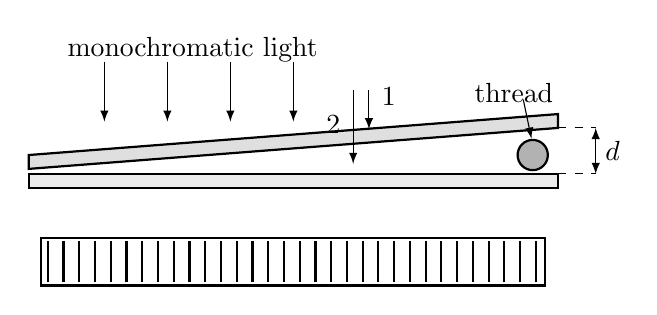
\begin{tikzpicture}[x=0.8cm,y=0.8cm,>=latex]
% lower plate
\draw[thick,fill=gray!15] (0,0) rectangle (8.4,0.22);
% upper plate (inclined)
\draw[thick,fill=gray!25] (0,0.30) -- (8.4,0.95) -- (8.4,1.17) -- (0,0.52) -- cycle;
% thread at the right end
\draw[thick,fill=gray!60] (8.0,0.52) circle (0.24);
\node at (7.7,1.5) {thread};
\draw[->] (7.85,1.4) -- (7.98,0.78);
% incident arrows
\foreach \x in {1.2,2.2,3.2,4.2} \draw[->] (\x,2.0) -- (\x,1.05);
\node at (2.6,2.2) {monochromatic light};
% beams 1 and 2
\draw[->] (5.4,1.55) -- (5.4,0.93);
\node[right] at (5.45,1.45) {$1$};
\draw[->] (5.15,1.55) -- (5.15,0.38);
\node[left] at (5.1,1.0) {$2$};
% d dimension at the right
\draw[<->] (9.0,0.22) -- (9.0,0.95) node[midway,right] {$d$};
\draw[dashed] (8.4,0.22) -- (9.0,0.22);
\draw[dashed] (8.4,0.95) -- (9.0,0.95);
% fringe pattern below
\begin{scope}[shift={(0.2,-1.55)}]
\draw[thick] (0,0) rectangle (8.0,0.75);
\foreach \x in {0.1,0.35,...,7.9} \draw[thick] (\x,0.05) -- (\x,0.70);
\end{scope}
\end{tikzpicture}
\end{figbox}

\subsection*{Experiment 8.18 \quad Measurement of the radius of curvature of a spherical surface with Newton's rings}

\textbf{[Apparatus and materials available]} Reading microscope, sodium lamp ($\lambda=589.3\,\mathrm{nm}$), glass plate, plano-convex lens and flat glass (the specimen under test).

\textbf{[Requirements]}

(1) Write down the formula for measuring the radius of curvature of a concave lens with Newton's rings.

(2) Briefly describe the experimental steps.

(3) Measure and calculate the radius of curvature of the concave lens.

\textbf{Solution 8.18}\quad \textbf{1.} A plano-convex (or plano-concave) lens of very long focal length is placed on a flat glass plate, with its convex surface in contact with the plane, so that a thin air layer is formed near the point of contact. Monochromatic light is incident from the front on the thin air layer; the light reflected from its upper and lower surfaces gives two coherent beams with a fixed path difference, and equal-thickness interference produces a set of bright and dark rings centred on the point of contact, namely Newton's rings, as shown in Figs.~(a) and (b).

The diameter $d_k$ of the $k$-th dark ring of Newton's rings is related to the radius of curvature $R$ of the convex surface of the plano-convex lens and to the wavelength $\lambda$ by
\begin{equation}
d_k=\sqrt{4kR\lambda}. \tag{1}
\end{equation}

\begin{figbox}{8.18(a)}
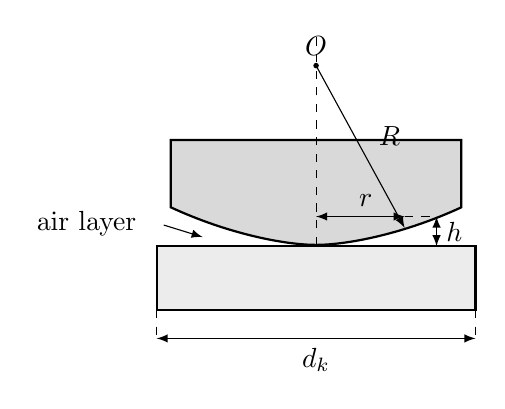
\begin{tikzpicture}[x=0.9cm,y=0.9cm,>=latex]
% flat glass
\draw[thick,fill=gray!15] (1.5,-0.9) rectangle (6.0,0);
% lens
\draw[thick,fill=gray!30] (1.7,1.5) -- (5.8,1.5) -- (5.8,0.55) .. controls (5.0,0.18) and (4.2,0.02) .. (3.75,0.02) .. controls (3.3,0.02) and (2.5,0.18) .. (1.7,0.55) -- cycle;
% air layer label (outside the lens)
\node[left] at (1.35,0.32) {air layer};
\draw[->] (1.6,0.30) -- (2.15,0.13);
% axis and centre of curvature
\draw[dashed] (3.75,0.02) -- (3.75,2.95);
\fill (3.75,2.55) circle (1pt) node[above] {$O$};
% R from O to the curved surface
\draw[->] (3.75,2.55) -- (5.0,0.26);
\node[right] at (4.5,1.55) {$R$};
% r at the air film
\draw[<->] (3.75,0.42) -- (5.0,0.42);
\node[above] at (4.45,0.42) {$r$};
% h
\draw[<->] (5.45,0) -- (5.45,0.42) node[midway,right] {$h$};
\draw[dashed] (5.0,0.42) -- (5.45,0.42);
% d_k
\draw[<->] (1.5,-1.3) -- (6.0,-1.3) node[midway,below] {$d_k$};
\draw[dashed] (1.5,-0.9) -- (1.5,-1.3);
\draw[dashed] (6.0,-0.9) -- (6.0,-1.3);
\end{tikzpicture}
\end{figbox}

\begin{figbox}{8.18(b)}
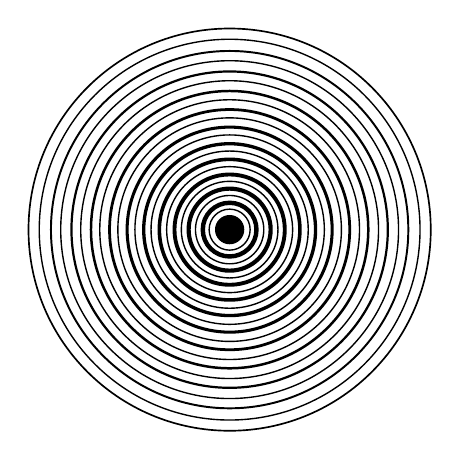
\begin{tikzpicture}[x=0.62cm,y=0.62cm]
% Newton's rings
\fill[black] (0,0) circle (0.30);
\foreach \rr/\w in {0.42/0.5,0.55/1.6,0.70/0.5,0.84/1.5,0.99/0.5,1.13/1.4,1.29/0.5,1.44/1.3,1.61/0.5,1.76/1.2,1.94/0.5,2.10/1.1,2.29/0.5,2.46/1.0,2.66/0.5,2.84/0.9,3.05/0.5,3.24/0.8,3.46/0.5,3.66/0.7,3.9/0.5,4.12/0.6}
  \draw[line width=\w pt] (0,0) circle (\rr);
\end{tikzpicture}
\end{figbox}

If $\lambda$ is known, then by measuring $d_k$ and reading off the order $k$ one can find the radius of curvature $R$.

Because the contact between the convex lens and the flat glass deforms the glass and so on, the centre of the rings is not necessarily a dark point, which makes the order $k$ difficult to determine correctly. In practice one usually measures the diameters $d_k$ and $d_{k+1}$ of two adjacent dark rings; from (1),
\begin{equation}
\Delta(d^2)=d_{k+1}^2-d_k^2=4R\lambda. \tag{2}
\end{equation}
To reduce the measurement error it is very necessary to make $\Delta(d^2)$ as large as possible. Usually the difference of the squares of the diameters of two dark rings separated by $m$ rings is used in the calculation:
\begin{equation}
\Delta(d^2)_m=d_{k+m}^2-d_k^2=4mR\lambda. \tag{3}
\end{equation}
The minus sign added here indicates that the order number of an outer ring is smaller than that of an inner ring (air gap between a plano-concave lens and a plane mirror).

\textbf{2. Experimental data and calculation}

\begin{center}
\textbf{Table 8.18}\quad Measurement of the diameters of Newton's rings\\[3pt]
\begin{tabular}{cccccc}
\toprule
Ring order & $x_{\text{left}}/\mathrm{mm}$ & $x_{\text{right}}/\mathrm{mm}$ & $d/\mathrm{mm}$ & $d^2/(\mathrm{mm})^2$ & $\Delta(d^2)_{20}/(\mathrm{mm})^2$ \\
\midrule
30 & 8.840 & 27.360 & 18.520 & 342.99 & \\
29 & 9.004 & 27.192 & 18.188 & 330.80 & \\
28 & 9.178 & 27.038 & 17.860 & 318.98 & \\
27 & 9.330 & 26.868 & 17.538 & 307.58 & \\
26 & 9.500 & 26.702 & 17.202 & 295.91 & \\
\midrule
10 & 12.848 & 23.352 & 10.504 & 110.33 & 232.66 \\
9 & 13.128 & 23.062 & 9.934 & 98.68 & 232.12 \\
8 & 13.430 & 22.750 & 9.320 & 86.86 & 232.12 \\
7 & 13.756 & 22.442 & 8.686 & 75.44 & 232.14 \\
6 & 14.110 & 22.084 & 7.974 & 63.58 & 232.33 \\
\bottomrule
\end{tabular}
\end{center}

From the table above,
\[
\Delta(d^2)=2.323\times10^{-4}\,\mathrm{m^2}.
\]
Therefore
\[
R=4.927\,\mathrm{m}.
\]

The following points must be noted in the measurement: (1) the ring number (order) of the interference fringes must not be miscounted; (2) during the measurement, vibrations of the table must be prevented from changing the interference rings; (3) in the measurement the crosshair must be aimed at the centre of the dark fringe of Newton's rings; (4) the screw-pitch error of the reading microscope must be eliminated; (5) in the experiment the measurement of a chord length may be used instead of the measurement of the diameter.

\begin{commentary}
This experiment enables students to understand, from experimental observation, the principle of equal-thickness interference and the concept of localised interference, to learn the use of the reading microscope, and to process the data by the method of successive differences so as to reduce the measurement error.
\end{commentary}

\subsection*{Experiment 8.19 \quad Measurement of the wavelength of light with a biprism}

\textbf{[Apparatus and materials available]} Optical bench, sodium lamp, adjustable slit (its holder can be translated and the slit can be rotated), biprism and its holder, convex lens, micrometer eyepiece, etc.

\textbf{[Requirements]}

(1) Write down the principle and the calculation formula for measuring the wavelength of light in the biprism interference experiment.

(2) Assemble the optical elements on the optical bench and adjust the interference fringes until clear fringes can be seen through the micrometer eyepiece; measure the fringe spacing $x$.

(3) Measure the separation $d$ of the two virtual sources by the two-image method.

(4) Measure the distance $D$ from the plane of the two virtual sources to the screen (the reticle of the micrometer eyepiece) and calculate the wavelength of the sodium light.

\textbf{Solution 8.19}\quad \textbf{1.} The Fresnel biprism is a thin glass plate whose upper surface is worked into two wedge-shaped faces with a very small wedge angle, the ridge being perpendicular to the end face, as shown in Fig.~1. The principle of the interference experiment with a biprism is shown in Fig.~2. A sodium lamp illuminates the slit $s$ (parallel to the ridge of the biprism). After the light wave emerging from the slit passes through the biprism $P$, its wavefront is divided into two parts, which propagate in different directions. These may be regarded as equivalent to the cylindrical waves emitted by two virtual sources $s_1$ and $s_2$ that satisfy the coherence conditions. If an observation screen is placed anywhere in the region where the two waves overlap, bright and dark interference fringes are seen, with their direction parallel to the slit. If the distance $d$ between $s_1$ and $s_2$, the distance $D$ from the plane containing $s_1$ and $s_2$ to the observation screen, and the fringe width $x$ are known, the wavelength $\lambda$ of the light source is given by
\[
\lambda=x\frac{d}{D}.
\]
Usually $D$ is several hundred millimetres, $d$ is about $1$--$2\,\mathrm{mm}$ and $x$ is about a few tenths of a millimetre. $D$ may be measured with a metre rule, $d$ by the two-image method with a convex lens and the micrometer eyepiece, and $x$ with the micrometer eyepiece. The wavelength $\lambda$ of the monochromatic light can then be found.

\begin{figbox}{8.19(a)}
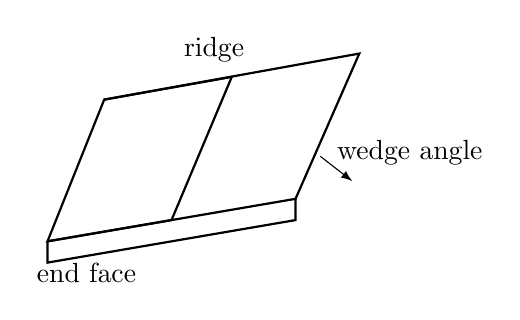
\begin{tikzpicture}[x=0.9cm,y=0.9cm,>=latex]
% plate in oblique projection
\coordinate (A) at (0.2,0.35);
\coordinate (B) at (3.7,0.95);
\coordinate (C) at (4.6,3.0);
\coordinate (D) at (1.0,2.35);
\coordinate (M) at (1.95,0.65);
\coordinate (N) at (2.8,2.67);
\draw[thick] (A) -- (B) -- (C) -- (D) -- cycle;
\draw[thick] (A) -- (M);
\draw[thick] (D) -- (N);
\draw[thick] (M) -- (N);
% end face shading
\draw[thick] (A) -- (0.2,0.05) -- (3.7,0.65) -- (B);
% labels
\node[above] at (2.55,2.75) {ridge};
\node[below] at (0.75,0.18) {end face};
\node[right] at (4.15,1.6) {wedge angle};
\draw[->] (4.05,1.55) -- (4.5,1.2);
\end{tikzpicture}
\end{figbox}

\begin{figbox}{8.19(b)}
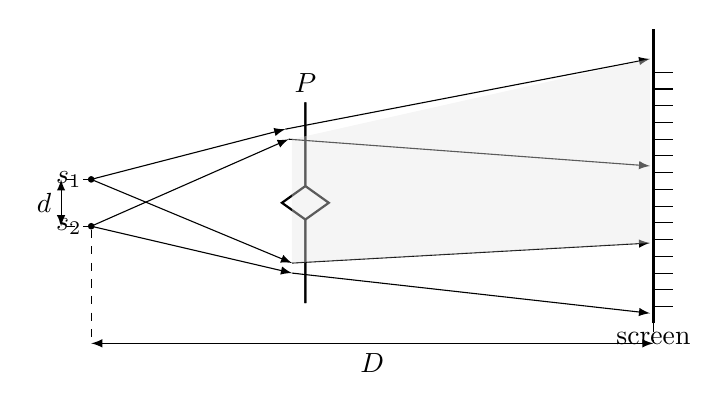
\begin{tikzpicture}[x=0.85cm,y=0.85cm,>=latex]
% screen
\draw[thick] (9.6,-1.8) -- (9.6,2.6);
\node[below] at (9.6,-1.8) {screen};
% biprism
\draw[thick] (4.4,-1.5) -- (4.4,-0.25) -- (4.75,0) -- (4.4,0.25) -- (4.4,1.5);
\draw[thick] (4.4,-1.5) -- (4.4,-0.25) -- (4.05,0) -- (4.4,0.25) -- (4.4,1.5);
\node[above] at (4.4,1.5) {$P$};
% virtual sources
\fill (1.2,0.35) circle (1.2pt) node[left] {$s_1$};
\fill (1.2,-0.35) circle (1.2pt) node[left] {$s_2$};
% d dimension
\draw[<->] (0.75,-0.35) -- (0.75,0.35) node[midway,left] {$d$};
\draw[dashed] (1.2,0.35) -- (0.75,0.35);
\draw[dashed] (1.2,-0.35) -- (0.75,-0.35);
% rays from s1 and s2 through biprism halves
\draw[->] (1.2,0.35) -- (4.1,1.1);
\draw[->] (4.1,1.1) -- (9.55,2.15);
\draw[->] (1.2,0.35) -- (4.2,-0.9);
\draw[->] (4.2,-0.9) -- (9.55,-0.6);
\draw[->] (1.2,-0.35) -- (4.15,0.95);
\draw[->] (4.15,0.95) -- (9.55,0.55);
\draw[->] (1.2,-0.35) -- (4.2,-1.05);
\draw[->] (4.2,-1.05) -- (9.55,-1.65);
% overlapping region shading
\fill[gray!20,opacity=0.4] (4.2,0.95) -- (9.55,2.15) -- (9.55,-0.6) -- (4.2,-0.9) -- cycle;
% fringes on screen
\foreach \y in {-1.55,-1.3,...,2.0} \draw (9.6,\y) -- (9.9,\y);
% D dimension
\draw[<->] (1.2,-2.1) -- (9.6,-2.1) node[midway,below] {$D$};
\draw[dashed] (1.2,-0.4) -- (1.2,-2.1);
\draw[dashed] (9.6,-1.8) -- (9.6,-2.1);
\end{tikzpicture}
\end{figbox}

\textbf{2. Experimental method}

(1) Adjusting the light path. Place the sodium lamp $N$, the slit $s$, the biprism $P$ and the micrometer eyepiece $E$ on the optical bench and make them coaxial, as shown in Fig.~3. First open the slit $s$ somewhat wide and adjust the left--right positions of the slit and of the eyepiece so that the region where the waves from the two virtual sources overlap lies within the aperture of the micrometer eyepiece. Then adjust the position of the sodium lamp so that the illumination on the two sides of the overlap region is equal. If interference fringes are to appear in the field of view of the eyepiece, the slit must first be made as narrow as possible, but not closed; at the same time the orientation of the slit must be rotated slowly, and when the slit is parallel to the ridge of the biprism clear interference fringes are seen.

\begin{figbox}{8.19(c)}
\begin{tikzpicture}[x=1.0cm,y=1.0cm,>=latex]
% ---------- top view ----------
\begin{scope}[yshift=2.6cm]
\draw[thick] (0,0) circle (0.22);
\node[below] at (0,-0.22) {$N$};
\draw[thick] (1.9,-0.45) -- (1.9,0.45);
\node[above] at (1.9,0.45) {$s$};
\draw[thick] (3.6,-0.35) -- (3.6,-0.1) -- (3.9,0) -- (3.6,0.1) -- (3.6,0.35);
\draw[thick] (3.6,-0.35) -- (3.6,-0.1) -- (3.3,0) -- (3.6,0.1) -- (3.6,0.35);
\node[above] at (3.6,0.35) {$P$};
\draw[thick] (6.4,-0.3) rectangle (7.6,0.3);
\draw[thick] (7.6,-0.15) rectangle (8.1,0.15);
\node[above] at (7.0,0.3) {$E$};
\draw[dashed] (-0.3,0) -- (8.3,0);
\node[left] at (-0.4,0.75) {top view};
\end{scope}
% ---------- side view ----------
\begin{scope}
\draw[thick] (0,-0.55) circle (0.2);
\node[left] at (-0.2,-0.55) {$N$};
\draw[thick] (1.9,-1.0) -- (1.9,0.35);
\node[above] at (1.9,0.35) {$s$};
\draw[thick] (3.6,-0.35) -- (3.6,-0.1) -- (3.9,0) -- (3.6,0.1) -- (3.6,0.35);
\draw[thick] (3.6,-0.35) -- (3.6,-0.1) -- (3.3,0) -- (3.6,0.1) -- (3.6,0.35);
\node[above] at (3.6,0.35) {$P$};
\draw[thick] (6.4,-0.3) rectangle (7.6,0.3);
\draw[thick] (7.6,-0.15) rectangle (8.1,0.15);
\node[above] at (7.0,0.3) {$E$};
\draw[dashed] (-0.3,0) -- (8.3,0);
\node[left] at (-0.4,0.75) {side view};
\end{scope}
\end{tikzpicture}
\end{figbox}

(2) Measure the width $x$ of the interference fringes with the micrometer eyepiece. Measure the total width of 10 (or 20) adjacent interference fringes and take the average as $x$.

(3) Measure the distance $D$ between the slit and the reticle of the micrometer eyepiece. Note that neither the slit nor the reticle lies in the same plane as the reading mark of its sliding carriage, so the value of $D$ must be corrected.

(4) Measure the distance $d$ between the two virtual sources by the two-image method. Make the distance between the reticle of the micrometer eyepiece and the slit slightly larger than $4f$, where $f$ is the focal length of the convex lens. Two images are formed, one magnified with size $d_1$ and the other reduced with size $d_2$; repeat five times and take the average. The separation of the two virtual sources $s_1$ and $s_2$ is then $d=\sqrt{d_1d_2}$.

\textbf{3. Experimental data and calculation}

\begin{center}
\textbf{Table 8.19-1}\quad Measurement of the fringe width $x$\\[3pt]
\begin{tabular}{ccccc}
\toprule
Order & Reading 1$/\mathrm{mm}$ & Order & Reading 2$/\mathrm{mm}$ & Width of 20 fringes $20x/\mathrm{mm}$ \\
\midrule
$k_1$ & 1.658 & $k_1+20$ & 6.182 & 4.524 \\
$k_2$ & 1.908 & $k_2+20$ & 6.400 & 4.492 \\
$k_3$ & 2.118 & $k_3+20$ & 6.642 & 4.524 \\
$k_4$ & 2.340 & $k_4+20$ & 6.878 & 4.538 \\
$k_5$ & 2.570 & $k_5+20$ & 7.084 & 4.514 \\
\bottomrule
\end{tabular}
\end{center}

\[
20\bar{x}=4.518\,\mathrm{mm};\qquad \bar{x}=0.2259\,\mathrm{mm}.
\]

The reading indicated on the carriage of the adjustable slit is $1240.0\,\mathrm{mm}$ (in fact the position of the slit is $1240.0\,\mathrm{mm}$ plus a correction of $42.5\,\mathrm{mm}$); the reading on the carriage of the micrometer eyepiece is $634.0\,\mathrm{mm}$ (in fact the position of the crosshair in the micrometer eyepiece is $634.0\,\mathrm{mm}$ plus a correction of $-27.0\,\mathrm{mm}$). Hence
\[
D=1240.0-634.0+42.5+27.0\approx676.0\ (\mathrm{mm}).
\]

\begin{center}
\textbf{Table 8.19-2}\quad Measurement of the separation of the virtual sources by the two-image method\\[3pt]
\begin{tabular}{ccccccc}
\toprule
Order & \multicolumn{3}{c}{Magnified image$/\mathrm{mm}$} & \multicolumn{3}{c}{Reduced image$/\mathrm{mm}$} \\
\cmidrule(lr){2-4}\cmidrule(lr){5-7}
 & Reading 1 & Reading 2 & $d_1/\mathrm{mm}$ & Reading 1 & Reading 2 & $d_2/\mathrm{mm}$ \\
\midrule
1 & 7.358 & 5.190 & & 6.370 & 4.950 & \\
2 & 7.376 & 5.210 & & 6.398 & 4.954 & \\
3 & 7.348 & 5.174 & & 6.400 & 4.960 & \\
4 & 7.362 & 5.188 & & 6.430 & 4.970 & \\
5 & 7.326 & 5.180 & & 6.412 & 4.972 & \\
\midrule
Average & 7.354 & 5.188 & 2.166 & 6.402 & 4.961 & 1.437 \\
\bottomrule
\end{tabular}
\end{center}

\[
d_1=2.166\,\mathrm{mm};\qquad d_2=1.437\,\mathrm{mm}.
\]

The wavelength of the sodium light is
\[
\lambda=\frac{x\sqrt{d_1d_2}}{D}=5896\ (\text{\AA})=589.6\ (\mathrm{nm}).
\]

\subsection*{Experiment 8.20 \quad Measurement of the grating constant by the principle of multiple-slit diffraction}

\textbf{[Apparatus and materials available]} Spectrometer, grating, mercury lamp, etc.

\textbf{[Requirements]}

(1) Adjust the spectrometer and write down the requirements for its adjustment.

(2) Adjust the platform screws so that the scratches of the grating are parallel to the axis of the spectrometer.

(3) Measure the data and calculate the grating constant of the grating.

\textbf{Solution 8.20}\quad \textbf{1.} Place the plane grating vertically on the object stage and make the plane of the grating coincide as nearly as possible with the perpendicular bisector of the line joining the platform adjusting screws $b$ and $c$. Using the reflection from the glass backing of the grating, adjust the spectrometer so that the telescope is focused at infinity, its optical axis is perpendicular to the axis of rotation of the spectrometer, and the plane of the grating is parallel to that axis. With the telescope already adjusted, adjust the collimator so that it emits parallel light and its optical axis is parallel to the optical axis of the telescope.

2. Adjust the platform screw $a$ so that the scratches of the grating are parallel to the axis of rotation of the spectrometer. The screws $a$, $b$ and $c$ are distributed on the platform as shown in the figure. The spectral lines seen through the telescope should then all lie at the same height. Finally, rotate the entrance slit of the collimator slightly until the spectral lines are parallel to the vertical crosshair of the telescope.

3. After the spectrometer has been adjusted, measure the diffraction angle $\varphi$ corresponding to the bright lines of the three spectral lines with $m=\pm1$, repeat the measurement five times and take the average. Substitute into the formula
\begin{equation}
d\sin\varphi=m\lambda\qquad(m=0,\pm1,\pm2,\ldots), \tag{1}
\end{equation}
where $d$ is the grating constant, $\lambda$ the wavelength of the light, and $m$ the order of the spectral line.

\begin{figbox}{8.20}
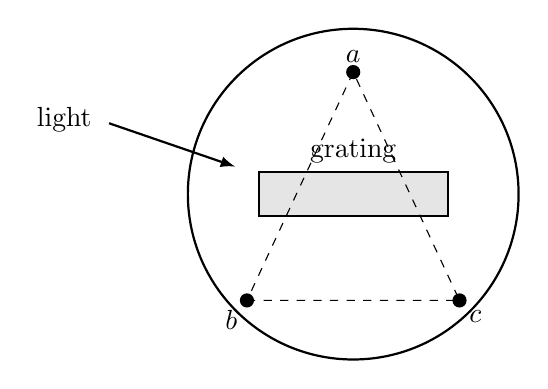
\begin{tikzpicture}[x=1.0cm,y=1.0cm,>=latex]
% platform
\draw[thick] (0,0) circle (2.1);
% grating
\draw[thick,fill=gray!20] (-1.2,-0.28) rectangle (1.2,0.28);
\node at (0,0.55) {grating};
% screws
\fill (-1.35,-1.35) circle (0.09) node[below left] {$b$};
\fill (1.35,-1.35) circle (0.09) node[below right] {$c$};
\fill (0,1.55) circle (0.09) node[above] {$a$};
% light beam
\draw[->,thick] (-3.1,0.9) -- (-1.5,0.35);
\node[left] at (-3.2,0.95) {light};
% dashed triangle of screws
\draw[dashed] (-1.35,-1.35) -- (1.35,-1.35) -- (0,1.55) -- cycle;
\end{tikzpicture}
\end{figbox}

\begin{center}
\textbf{Table 8.20-1}\quad Positions of the zeroth-order and $\pm1$-order diffracted lines\\[3pt]
{\footnotesize\setlength{\tabcolsep}{3.5pt}
\begin{tabular}{ccccccc}
\toprule
$\lambda/\mathrm{nm}$ & \multicolumn{2}{c}{Zeroth order} & \multicolumn{2}{c}{$+1$ order} & \multicolumn{2}{c}{$-1$ order} \\
\cmidrule(lr){2-3}\cmidrule(lr){4-5}\cmidrule(lr){6-7}
 & window ``1'' & window ``2'' & window ``2'' & window ``1'' & window ``1'' & window ``2'' \\
\midrule
546.07 (green) & $223\degree13'$ & $43\degree13.5'$ & $215\degree22'$ & $35\degree23'$ & $231\degree4.5'$ & $51\degree5.5'$ \\
 & $223\degree13.5'$ & $43\degree14.5'$ & $215\degree22'$ & $35\degree23'$ & $231\degree4.5'$ & $51\degree5.5'$ \\
 & $223\degree13'$ & $43\degree13.5'$ & $215\degree22'$ & $35\degree22.5'$ & $231\degree5'$ & $51\degree6'$ \\
 & $223\degree12.5'$ & $43\degree13.5'$ & $215\degree22.5'$ & $35\degree22.5'$ & $231\degree4.5'$ & $51\degree5.5'$ \\
 & $223\degree12.5'$ & $43\degree13.5'$ & $215\degree22.5'$ & $35\degree23'$ & $231\degree5'$ & $51\degree5.5'$ \\
\midrule
576.96 (yellow) & & & $214\degree55'$ & $34\degree55.5'$ & $231\degree31'$ & $51\degree32'$ \\
 & & & $214\degree54.5'$ & $34\degree55.5'$ & $231\degree31'$ & $51\degree31.5'$ \\
 & & & $214\degree54.5'$ & $34\degree55'$ & $231\degree31.5'$ & $51\degree32'$ \\
 & & & $214\degree54.5'$ & $34\degree55.5'$ & $231\degree31'$ & $51\degree32'$ \\
 & & & $214\degree55'$ & $34\degree55.5'$ & $231\degree31.5'$ & $51\degree32.5'$ \\
\bottomrule
\end{tabular}
}
\end{center}

\begin{center}
\textbf{Table 8.20-2}\quad Data and calculated results\\[3pt]
\begin{tabular}{ccc}
\toprule
$\lambda/\mathrm{nm}$ & $\varphi$ & $d/\mathrm{nm}$ \\
\midrule
546.07 & $7\degree51.3'$ & 3996 \\
576.96 & $8\degree18.3'$ & 3994 \\
\bottomrule
\end{tabular}
\end{center}

$\lambda=576.96\,\mathrm{nm}$ is the shorter-wavelength line of the yellow doublet.

The grating constant is $d=3995\,\mathrm{nm}$.

\subsection*{Experiment 8.21 \quad Observation of single-slit and single-thread diffraction, and measurement of the slit width and the thread diameter}

\textbf{[Apparatus and materials available]} Optical bench, sliders, single slit and its holder, single fine thread and its holder, white screen, ruler and semiconductor laser.

\textbf{[Requirements]}

(1) Briefly describe the principle of single-slit diffraction and write down the single-slit diffraction formula.

(2) Measure the width of the single slit and the diameter of the fine thread.

\textbf{Solution 8.21}\quad \textbf{1.} By Fraunhofer diffraction, parallel light from the source falls perpendicularly on the single slit (or single thread). According to the Huygens--Fresnel principle, every point of the slit may be regarded as a new source emitting spherical waves in all directions, and the waves superpose on the receiving screen to form a set of bright and dark fringes parallel to the slit. In experiments the parallel light is obtained either by placing the source at infinity or by means of two convex lenses; when a laser is used as the source, the two lenses may be omitted because of the collimation of the laser beam. The experimental light path is as shown in the figure.

When the distance $Z$ from the slit to the screen is much greater than $a$, where $a$ is the slit width, the angle $\theta$ is very small, and then $\sin\theta\approx\tan\theta=x_k/Z$. The diffraction angles of the dark fringes of various orders are
\begin{equation}
\sin\theta=\frac{K\lambda}{a}\approx\frac{x_k}{Z},\qquad K=0,1,2,3,\ldots \tag{1}
\end{equation}
Hence the width of the single slit is
\begin{equation}
a=\frac{K\lambda Z}{x_k}, \tag{2}
\end{equation}
where $K$ is the order of the dark fringe, $Z$ the distance from the slit to the screen, and $x_k$ the distance of the $K$-th order dark fringe from the centre of the central maximum.

If a single thread replaces the single slit, formulas (1) and (2) still hold.

\textbf{2. Experimental data}

The data for the single slit are given in Table 1; the wavelength of the semiconductor laser is $\lambda=650.0\,\mathrm{nm}$.

\begin{center}
\textbf{Table 8.21-1}\\[3pt]
\begin{tabular}{cccc}
\toprule
$K$ & $Z/\mathrm{cm}$ & $\bar{x}_k/\mathrm{cm}$ & $a/\mathrm{mm}$ \\
\midrule
4 & 102.0 & 0.82 & 0.323 \\
\bottomrule
\end{tabular}
\end{center}

The slit width measured with a JCD3 reading microscope is $\bar{a}=0.324\,\mathrm{mm}$, which is quite close to the above value.

The measurements of the thread diameter are given in Table 2.

\begin{center}
\textbf{Table 8.21-2}\\[3pt]
\begin{tabular}{cccc}
\toprule
$K$ & $Z/\mathrm{cm}$ & $\bar{x}_k/\mathrm{cm}$ & $a/\mathrm{mm}$ \\
\midrule
5 & 102.0 & 1.95 & 0.170 \\
10 & 102.0 & 3.92 & 0.169 \\
\bottomrule
\end{tabular}
\end{center}

\begin{figbox}{8.21}
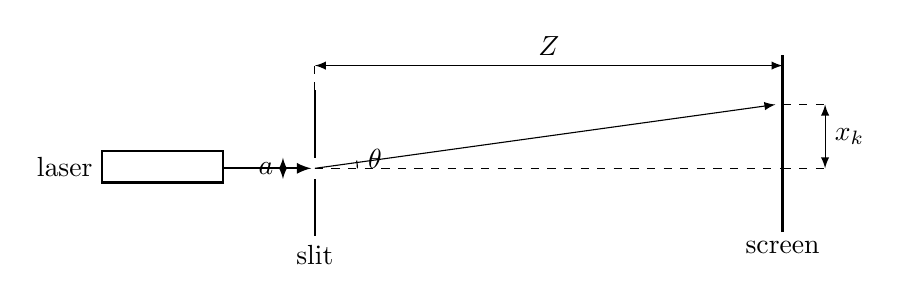
\begin{tikzpicture}[x=0.9cm,y=0.9cm,>=latex]
% laser
\draw[thick] (0,0.8) rectangle (1.7,1.25);
\node[left] at (0,1.02) {laser};
% slit plane
\draw[thick] (3.0,0.05) -- (3.0,0.85);
\draw[thick] (3.0,1.15) -- (3.0,2.1);
\node[below] at (3.0,0.05) {slit};
% a dimension
\draw[<->] (2.55,0.85) -- (2.55,1.15) node[midway,left] {$a$};
% beam
\draw[->,thick] (1.7,1.0) -- (2.95,1.0);
% axis
\draw[dashed] (3.0,1.0) -- (9.6,1.0);
% diffracted ray to x_k
\draw[->] (3.0,1.0) -- (9.5,1.9);
\draw (3.6,1.0) arc (0:10.6:0.6);
\node at (3.85,1.13) {$\theta$};
% screen
\draw[thick] (9.6,0.1) -- (9.6,2.6);
\node[below] at (9.6,0.1) {screen};
% x_k
\draw[<->] (10.2,1.0) -- (10.2,1.9) node[midway,right] {$x_k$};
\draw[dashed] (9.6,1.0) -- (10.2,1.0);
\draw[dashed] (9.6,1.9) -- (10.2,1.9);
% Z dimension
\draw[<->] (3.0,2.45) -- (9.6,2.45) node[midway,above] {$Z$};
\draw[dashed] (3.0,2.1) -- (3.0,2.45);
\draw[dashed] (9.6,2.6) -- (9.6,2.45);
\end{tikzpicture}
\end{figbox}

The average diameter of the single thread measured with the reading microscope is $\bar{x}=0.167\,\mathrm{mm}$; the percentage difference between the two values is $1.8\%$.

\subsection*{Experiment 8.22 \quad Assembly of a telescope and measurement of its magnifying power}

\textbf{[Apparatus and materials available]} Optical bench, two convex lenses (one of focal length $200$--$250\,\mathrm{mm}$, the other of $20$--$25\,\mathrm{mm}$), one metre rule.

\textbf{[Requirements]}

(1) Draw the measuring light path and assemble a Kepler telescope.

(2) Write down the measuring method and the experimental steps.

(3) Measure the magnifying power of the self-assembled telescope.

\textbf{Solution 8.22}\quad \textbf{1.} Use the converging lens of focal length $200$--$250\,\mathrm{mm}$ as the objective and the converging lens of focal length $20$--$25\,\mathrm{mm}$ as the eyepiece. Mount them on an optical bench as shown in the figure, with the distance between the objective and the eyepiece equal to the sum of the two focal lengths, and adjust them until they are coaxial. A Kepler telescope is thus assembled.

2. Place a metre rule in a plane perpendicular to the optical axis at a large distance (greater than $2\,\mathrm{m}$). The experimenter observes the metre rule through the self-assembled telescope with one eye and looks at the distant metre rule directly with the other eye; the visual system then superimposes the two images. Adjust the distance between the objective and the eyepiece slightly until there is no parallax between the two images. The reciprocal of the ratio of a fixed graduation value on the image of the metre rule magnified by the telescope (for example the image of a 1 cm interval) to the graduation value seen directly by the eye on the metre rule is the magnifying power $M$ of the self-assembled telescope.

The main source of measurement error is that the metre rule is not placed at infinity but at a finite distance $S$ from the objective of the telescope. If the focal length of the objective is $f_0$ and that of the eyepiece is $f_e$, the magnifying power of the telescope focused at infinity is $M=\dfrac{f_0}{f_e}$. If it is focused at the finite distance $S$, its magnifying power $M'$ must be corrected as follows:
\[
M'=M\frac{S}{S+f_0}.
\]

\begin{figbox}{8.22}
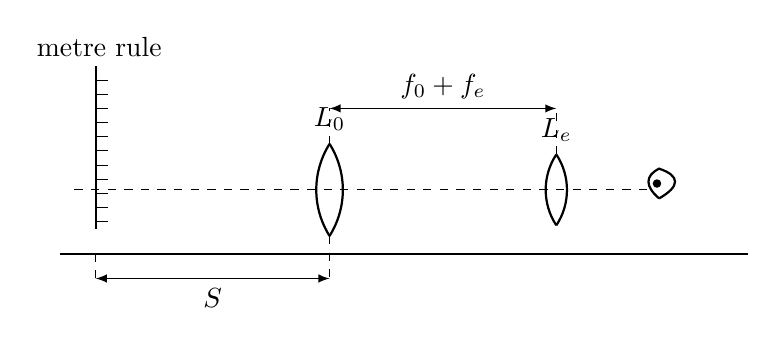
\begin{tikzpicture}[x=0.9cm,y=0.9cm,>=latex]
% bench
\draw[thick] (0.6,-0.9) -- (10.3,-0.9);
% ruler at the left
\draw[thick] (1.1,-0.55) -- (1.1,1.75);
\foreach \y in {-0.45,-0.25,...,1.65} \draw (1.1,\y) -- (1.28,\y);
\node[above] at (1.15,1.75) {metre rule};
% objective
\draw[thick] (4.4,-0.65) .. controls (4.65,-0.25) and (4.65,0.25) .. (4.4,0.65);
\draw[thick] (4.4,-0.65) .. controls (4.15,-0.25) and (4.15,0.25) .. (4.4,0.65);
\node[above] at (4.4,0.7) {$L_0$};
% eyepiece
\draw[thick] (7.6,-0.5) .. controls (7.8,-0.2) and (7.8,0.2) .. (7.6,0.5);
\draw[thick] (7.6,-0.5) .. controls (7.4,-0.2) and (7.4,0.2) .. (7.6,0.5);
\node[above] at (7.6,0.55) {$L_e$};
% axis
\draw[dashed] (0.8,0) -- (8.9,0);
% eye
\draw[thick] (9.05,-0.12) .. controls (9.35,0.05) and (9.35,0.2) .. (9.05,0.3) .. controls (8.85,0.2) and (8.85,0.05) .. (9.05,-0.12);
\fill (9.02,0.09) circle (0.06);
% S dimension
\draw[<->] (1.1,-1.25) -- (4.4,-1.25) node[midway,below] {$S$};
\draw[dashed] (1.1,-0.9) -- (1.1,-1.25);
\draw[dashed] (4.4,-0.65) -- (4.4,-1.25);
% f0+fe
\draw[<->] (4.4,1.15) -- (7.6,1.15) node[midway,above] {$f_0+f_e$};
\draw[dashed] (4.4,0.65) -- (4.4,1.15);
\draw[dashed] (7.6,0.5) -- (7.6,1.15);
\end{tikzpicture}
\end{figbox}

\subsection*{Experiment 8.23 \quad Assembly of a microscope and measurement of its magnifying power}

\textbf{[Apparatus and materials available]} Optical bench, small electric bulb, ground glass, a millimetre scale ruled on a transparent plate, convex lens (focal length $40$--$50\,\mathrm{mm}$), convex lens (focal length $25\,\mathrm{mm}$), semi-transparent semi-reflecting mirror, metre rule, lens holders, supports, illuminating lamp, etc.

\textbf{[Requirements]}

(1) Assemble a microscope with the apparatus supplied.

(2) Measure the magnifying power $M$ of the assembled microscope.

\textbf{Solution 8.23}\quad \textbf{1.} Use the convex lens of focal length $40$--$50\,\mathrm{mm}$ as the objective and the convex lens of focal length $25\,\mathrm{mm}$ as the eyepiece, with an optical interval of $170\,\mathrm{mm}$ (the optical interval is the distance from the second focal point of the objective to the first focal point of the eyepiece). Place them on the optical bench to form a microscope, as shown in the figure.

2. From left to right, place the small electric bulb, the ground glass and the transparent plate (bearing the millimetre scale) in front of the objective. Behind the eyepiece place a semi-transparent semi-reflecting mirror (a plane glass plate coated with a chromium film) whose reflectance is $50\%$, inclined at $45\degree$ to the principal axis. At a distance of about $250\,\mathrm{mm}$ from the semi-transparent semi-reflecting mirror, in the direction perpendicular to the optical axis, place a metre rule illuminated by the light source (the illuminating lamp), as shown in the figure. When the light source illuminates the millimetre scale through the ground glass, the experimenter can observe simultaneously with the eye the virtual image of the millimetre scale formed by the assembled microscope and the virtual image of the metre rule formed by the semi-transparent semi-reflecting mirror. When the two images are adjusted until no parallax exists between them, the magnifying power $M$ of the assembled microscope can be found from the ratio of their sizes.

\begin{figbox}{8.23}
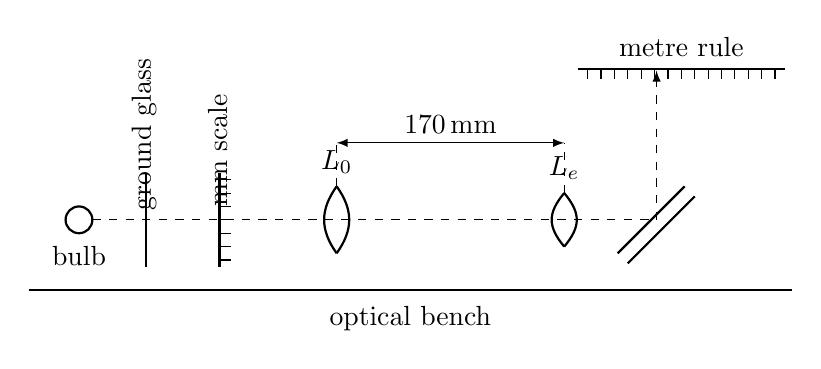
\begin{tikzpicture}[x=0.85cm,y=0.85cm,>=latex]
% bench
\draw[thick] (0,0) -- (11.4,0);
\node[below] at (5.7,-0.1) {optical bench};
% lamp
\draw[thick] (0.75,1.05) circle (0.2);
\node[below] at (0.75,0.8) {bulb};
% ground glass
\draw[thick] (1.75,0.35) -- (1.75,1.75);
\node[right,rotate=90] at (1.72,1.05) {ground glass};
% millimetre scale plate
\draw[thick] (2.85,0.35) -- (2.85,1.75);
\foreach \y in {0.45,0.65,...,1.7} \draw (2.85,\y) -- (3.02,\y);
\node[right,rotate=90] at (2.82,1.1) {mm scale};
% objective
\draw[thick] (4.6,0.55) .. controls (4.85,0.9) and (4.85,1.2) .. (4.6,1.55);
\draw[thick] (4.6,0.55) .. controls (4.35,0.9) and (4.35,1.2) .. (4.6,1.55);
\node[above] at (4.6,1.6) {$L_0$};
% eyepiece
\draw[thick] (8.0,0.65) .. controls (8.25,0.95) and (8.25,1.15) .. (8.0,1.45);
\draw[thick] (8.0,0.65) .. controls (7.75,0.95) and (7.75,1.15) .. (8.0,1.45);
\node[above] at (8.0,1.5) {$L_e$};
% optical interval
\draw[<->] (4.6,2.2) -- (8.0,2.2) node[midway,above] {$170\,\mathrm{mm}$};
\draw[dashed] (4.6,1.55) -- (4.6,2.2);
\draw[dashed] (8.0,1.45) -- (8.0,2.2);
% beam splitter at 45 degrees
\draw[thick] (8.8,0.55) -- (9.8,1.55);
\draw[thick] (8.95,0.4) -- (9.95,1.4);
% metre rule above
\draw[thick] (8.2,3.3) -- (11.3,3.3);
\foreach \x in {8.35,8.55,...,11.15} \draw (\x,3.3) -- (\x,3.15);
\node[above] at (9.75,3.35) {metre rule};
% reflected beam upwards to the rule
\draw[dashed,->] (9.38,1.05) -- (9.38,3.28);
% axis
\draw[dashed] (0.95,1.05) -- (9.35,1.05);
\end{tikzpicture}
\end{figbox}

\subsection*{Experiment 8.24 \quad Measurement of the relation between the emergent intensity $I$ of a ``polarised-light intensity regulator'' and the angle of rotation $\theta$}

Light is an electromagnetic wave; its electric and magnetic vectors are mutually perpendicular and both are perpendicular to the direction of propagation. Usually the electric vector is used to represent the light vector. In a plane perpendicular to the direction of propagation the light vector may have various states of oscillation; these are called the polarisation states of light. If the direction of the light vector is arbitrary and the average magnitude of the light vector is the same in all directions, the light is called natural light. If the direction of the light vector never changes and only its amplitude changes with a phase shift, so that the end point of the light vector traces a straight line, the light is called linearly polarised light or plane-polarised light. A device that converts natural light into polarised light is called a polariser; a device used to examine whether light is polarised is called an analyser. Polariser and analyser are collectively called polaroids.

Consider a beam of natural light which, after passing through two polaroids making a certain angle $\theta$ with each other, has an emergent intensity related to the angle $\theta$ by the following relation:
\[
I=DI_0\cos^n\theta,
\]
where $I_0$ is the intensity of the polarised light incident on the analyser and is a definite value once the instrument is fixed, $D$ is the transmittance of the analyser, and $n$ is a coefficient to be determined. Using the apparatus supplied, measure the relation between $I$ and $\theta$, and fit the above relation by a curve.

\textbf{[Apparatus and materials available]} Two polaroids with graduated discs, optical bench, one laser and its power supply, optical power meter with a silicon photocell, graph paper, etc.

\textbf{[Requirements]}

(1) The direction of the optical axis of a polaroid is not necessarily at the $\theta=0\degree$ position of the graduated disc; the directions of the optical axes of the two polaroids must be measured by the experimenter. (The laser beam emitted by the semiconductor laser is partially polarised.)

(2) Draw the experimental arrangement and measure the data of the $I$--$\theta$ relation.

(3) Find the coefficient $n$ to be determined by a graphical method.

(4) Write down the functional relation between $I$ and $\theta$.

\textbf{Solution 8.24}\quad \textbf{1.} Let the beam emitted by the laser be perpendicular to the centres of the polariser and the analyser and be incident perpendicularly on the silicon photocell of the optical power meter. Measure the light intensity $I$ with the optical power meter, read the angle $\theta$ on the graduated disc of the analyser, and measure the relation between $I$ and $\theta$.

2. Turn the disc of the analyser slowly, that is, change the direction of the optical axis of the analyser. When the reading of the optical power meter reaches its minimum or zero, the optical axis of the analyser is perpendicular to that of the polariser. Taking logarithms of both sides of the formula $I=DI_0\cos^n\theta$ gives
\[
\ln I=\ln DI_0+n\ln\cos\theta.
\]
Plot $\ln I$ against $\ln\cos\theta$; the slope of the straight line is the coefficient $n$ to be determined.

\textbf{3. Experimental data}

\begin{center}
\textbf{Table 8.24-1}\\[3pt]
\begin{tabular}{ccccccc}
\toprule
$\theta/\degree$ & 4.5 & 15.5 & 24.5 & 35.5 & 44.5 & 55.5 \\
\midrule
$I/\mathrm{mW}$ & 1.710 & 1.587 & 1.431 & 1.129 & 0.870 & 0.550 \\
\bottomrule
\end{tabular}
\end{center}

\begin{center}
\textbf{Table 8.24-2}\\[3pt]
\begin{tabular}{ccccccc}
\toprule
$\ln\cos\theta$ & $-3.09\times10^{-3}$ & $-0.0370$ & $-0.0944$ & $-0.206$ & $-0.338$ & $-0.568$ \\
\midrule
$\ln I$ & 0.536 & 0.462 & 0.358 & 0.121 & $-0.139$ & $-0.598$ \\
\bottomrule
\end{tabular}
\end{center}

Linear regression of the data in Table 2 gives the slope $n=2.007$ and the correlation coefficient $r=0.99994$. The graphical method gives the slope of the straight line as $n=2.01$, so $n\approx2$ (the graph is omitted).

The fitted empirical formula is
\[
I=1.710\cos^2\theta\quad(\text{unit: mW}).
\]
The diagram of the experimental arrangement is omitted.

\begin{commentary}
The results of this experiment verify Malus's law. This law shows that an analyser may be used as a device for adjusting the intensity of the incident polarised light; moreover, Malus's law may also be used to test whether the output working state of a silicon photocell is linear in the light intensity.
\end{commentary}

\subsection*{Experiment 8.25 \quad Measurement of the refractive index of semiconductor silicon by the extrapolation method}

\textbf{[Brief introduction to the principle]}

When light falls on the surface of a semiconductor, part of it is reflected, part absorbed and part transmitted. The ratio $R$ of the reflected light power $I_r$ to the incident light power $I_i$ is called the reflectance, that is,
\begin{equation}
R=\frac{I_r}{I_i}. \tag{1}
\end{equation}
The incident light may be resolved into two polarisation components: the component $P$ with its polarisation parallel to the plane of incidence, and the component $S$ with its polarisation perpendicular to the plane of incidence. In this experiment a semiconductor laser of wavelength $650\,\mathrm{nm}$ is used, and its absorption in the silicon surface may be neglected. Under this condition the reflectances $R_P$ and $R_S$ for light incident from air onto the surface of the material are given by the Fresnel formulas
\begin{align}
\pm\sqrt{R_P}&=\frac{n\cos\theta_i-\cos\theta_t}{\cos\theta_i+n\cos\theta_t}, \tag{2}\\
-\sqrt{R_S}&=\frac{\cos\theta_i-n\cos\theta_t}{\cos\theta_i+n\cos\theta_t}, \tag{3}
\end{align}
where $n$ is the refractive index of the material, $\theta_i$ the angle of incidence, $\theta_r$ the angle of reflection and $\theta_t$ the angle of refraction, as shown in Fig.~1.

At $\theta_i=0$ it is in practice impossible to measure $R_P$ and $R_S$ directly. The Fresnel formulas, however, allow $n$ to be calculated from the values of $R_P$ and $R_S$ obtained at an arbitrary angle of incidence.

\begin{figbox}{8.25(a)}
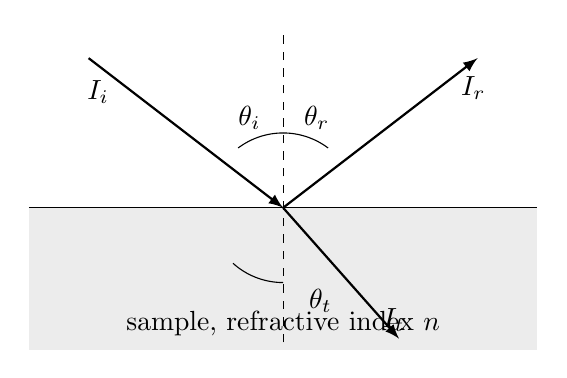
\begin{tikzpicture}[x=0.95cm,y=0.95cm,>=latex]
% surface
\draw[thick] (-3.4,0) -- (3.4,0);
\fill[gray!15] (-3.4,-1.9) rectangle (3.4,0);
\node at (0,-1.55) {sample, refractive index $n$};
% normal
\draw[dashed] (0,-1.8) -- (0,2.4);
% incident ray
\draw[->,thick] (-2.6,2.0) -- (0,0);
\node[left] at (-2.2,1.55) {$I_i$};
% reflected ray
\draw[->,thick] (0,0) -- (2.6,2.0);
\node[right] at (2.25,1.6) {$I_r$};
% refracted ray
\draw[->,thick] (0,0) -- (1.55,-1.75);
\node[right] at (1.2,-1.5) {$I_t$};
% angles
\draw (0,1.0) arc (90:127:1.0);
\node at (-0.45,1.2) {$\theta_i$};
\draw (0,1.0) arc (90:53:1.0);
\node at (0.45,1.2) {$\theta_r$};
\draw (0,-1.0) arc (270:228:1.0);
\node at (0.5,-1.25) {$\theta_t$};
\end{tikzpicture}
\end{figbox}

\textbf{[Apparatus and materials available]} The experimental arrangement is shown in Fig.~2.

(1) A semiconductor laser and its power supply, fixed on a rotating stage. The laser wavelength is $650\,\mathrm{nm}$.

(2) A linear polaroid of diameter $20\,\mathrm{mm}$, fixed on a rotating stage. Note that the zero reading of the stage is not necessarily the direction of the polarisation axis of the polaroid.

(3) A glass plate (refractive index $1.57$ at the wavelength $650\,\mathrm{nm}$) and a thin semiconductor silicon wafer (the sample), fixed on opposite sides of a rectangular metal block (the sample block).

(4) An optical rotating stage on which the sample block can be fixed.

(5) A digital laser power meter connected to a photodetector fixed on a support that can rotate about the sample.

(6) An optical bench, a light shield, graph paper, a flashlight and a soft tape, etc.

\begin{figbox}{8.25(b)}
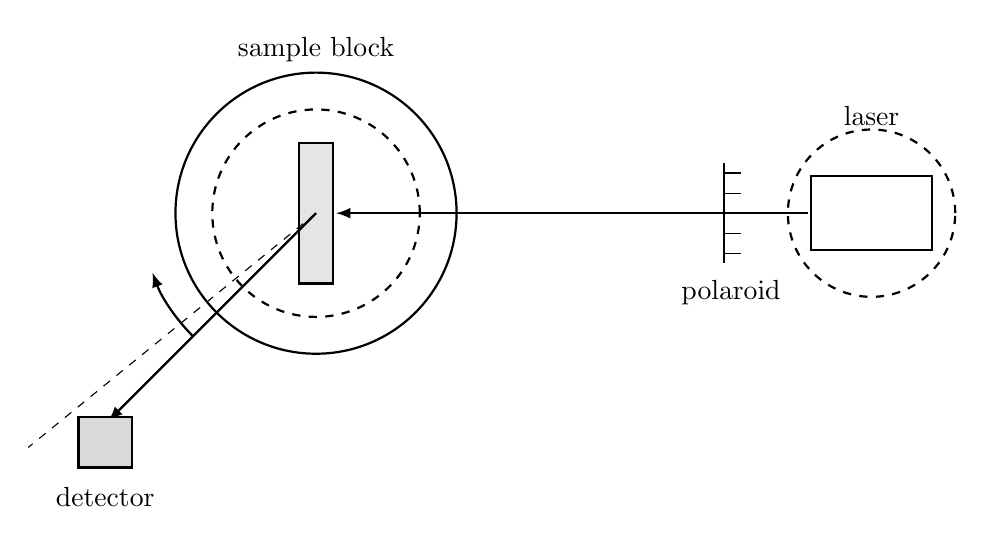
\begin{tikzpicture}[x=0.85cm,y=0.85cm,>=latex]
% rotating stage of the sample
\draw[thick] (0,0) circle (2.1);
\draw[thick,dashed] (0,0) circle (1.55);
% sample block
\draw[thick,fill=gray!20] (-0.25,-1.05) rectangle (0.25,1.05);
\node at (0,2.45) {sample block};
% laser on its stage at the right
\draw[thick] (7.4,-0.55) rectangle (9.2,0.55);
\node at (8.3,1.45) {laser};
\draw[thick,dashed] (8.3,0) circle (1.25);
% polarizer
\draw[thick] (6.1,-0.75) -- (6.1,0.75);
\foreach \y in {-0.6,-0.3,0,0.3,0.6} \draw (6.1,\y) -- (6.35,\y);
\node[below] at (6.2,-0.85) {polaroid};
% beam from laser to sample
\draw[->,thick] (7.35,0) -- (0.3,0);
% reflected beam to detector at lower left
\draw[->,thick] (0,0) -- (-3.1,-3.1);
% detector
\draw[thick,fill=gray!30] (-3.55,-3.8) rectangle (-2.75,-3.05);
\node[below] at (-3.15,-3.95) {detector};
% rotating arm for the detector
\draw[dashed] (0,0) -- (-4.3,-3.5);
\draw[thick,->] (0,0) ++(225:2.6) arc (225:200:2.6);
\end{tikzpicture}
\end{figbox}

\textbf{[Requirements]}

(1) Determine the plane of polarisation of the incident laser light.

In the experiment the polarisation axis of the polaroid should coincide with the direction of the strongest linear polarisation of the laser light.

(2) Measure the reflectances $R_P$ and $R_S$ of the thin semiconductor silicon wafer.

(3) Calculate the refractive index $n$ of the semiconductor silicon material.

\textbf{Solution 8.25}\quad \textbf{1.} In this experiment the plane of polarisation of the incident laser light must first be determined. It should be noted that the light emitted by a semiconductor laser is partially polarised. To obtain the best results in the experiment, the polarisation axis of the polaroid is made to coincide with the strongest component of the laser light. The laser, the polaroid and the detector are placed on one straight line. Fix either the laser or the polaroid and rotate the other; observe the light intensity measured by the photodetector until the intensity reaches its maximum. In the subsequent measurements the polaroid and the laser are treated as one system and are rotated together when necessary.

From the refractive index of the glass, the Brewster angle of the glass is calculated by the formula
\begin{equation}
\theta_B=\arctan n. \tag{4}
\end{equation}
The glass sample is fixed on the rotating stage at this position. Rotate the polarising system and measure the power of the reflected laser light at different polarisation angles. The experimental results are shown in Fig.~3. From them the angle of the polaroid relative to the incident glass sample at which the reflected laser power is minimum can be found. According to Brewster's principle, the plane of polarisation of the laser light is then parallel to the plane of incidence on the sample.

\begin{figbox}{8.25(c)}
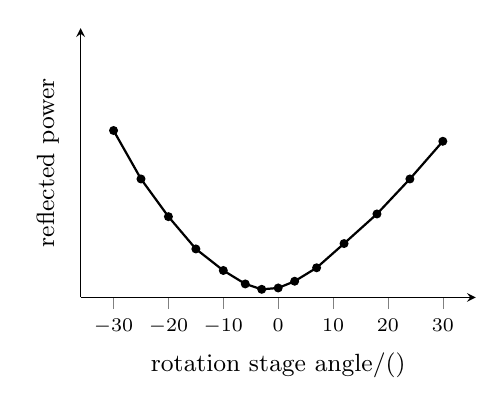
\begin{tikzpicture}
\begin{axis}[width=6.6cm,height=5.0cm,
  xlabel={rotation stage angle/$(\degree)$},ylabel={reflected power},
  xmin=-36,xmax=36,ymin=0,ymax=1.0,
  xtick={-30,-20,-10,0,10,20,30},
  ytick=\empty,
  axis lines=left, tick align=outside,
  label style={font=\small}, tick label style={font=\scriptsize}]
\addplot[thick,mark=*,mark size=1.2pt] coordinates {
(-30,0.62)(-25,0.44)(-20,0.30)(-15,0.18)(-10,0.10)(-6,0.05)(-3,0.03)(0,0.035)(3,0.06)(7,0.11)(12,0.20)(18,0.31)(24,0.44)(30,0.58)};
\end{axis}
\end{tikzpicture}
\end{figbox}

\begin{figbox}{8.25(d)}
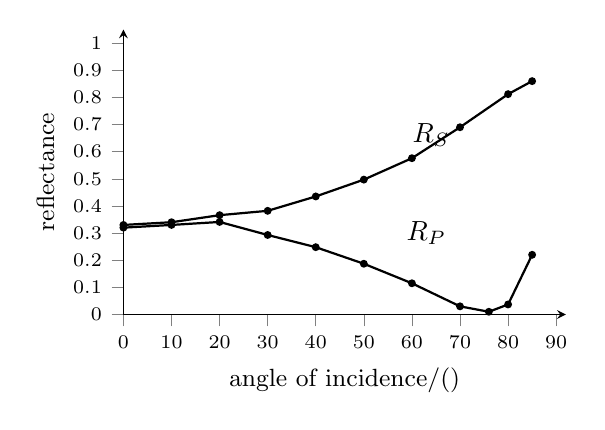
\begin{tikzpicture}
\begin{axis}[width=7.2cm,height=5.2cm,
  xlabel={angle of incidence/$(\degree)$},ylabel={reflectance},
  xmin=0,xmax=92,ymin=0,ymax=1.05,
  xtick={0,10,20,30,40,50,60,70,80,90},
  ytick={0,0.1,0.2,0.3,0.4,0.5,0.6,0.7,0.8,0.9,1.0},
  axis lines=left, tick align=outside,
  label style={font=\small}, tick label style={font=\scriptsize}]
\addplot[thick,mark=*,mark size=1pt] coordinates {
(0,0.32)(10,0.33)(20,0.341)(30,0.293)(40,0.248)(50,0.187)(60,0.115)(70,0.030)(76,0.010)(80,0.037)(85,0.22)};
\node at (axis cs:63,0.30) {$R_P$};
\addplot[thick,mark=*,mark size=1pt] coordinates {
(0,0.33)(10,0.34)(20,0.366)(30,0.382)(40,0.435)(50,0.497)(60,0.576)(70,0.69)(80,0.812)(85,0.86)};
\node at (axis cs:64,0.66) {$R_S$};
\end{axis}
\end{tikzpicture}
\end{figbox}

2. With the direction of the plane of polarisation of the laser light determined as above, make it perpendicular and parallel respectively to the plane of incidence on the semiconductor silicon, and measure the reflected laser power at different angles, as shown in Fig.~4. In this figure the relations $R_P$--$\theta_i$ and $R_S$--$\theta_i$ are extrapolated to the reflectance at zero angle of incidence; the two should converge to one point.

When plotting, take care to measure more points near the minimum so as to ensure that the graph is smooth and correct.

3. The average of several measured values of the refractive index $n$ is given in the table below.

\begin{center}
\textbf{Table 8.25}\\[3pt]
\begin{tabular}{ccccc}
\toprule
$\theta_i/(\degree)$ & $R_P$ & $R_S$ & $n$ & $\bar{n}$ \\
\midrule
20.0 & 0.341 & 0.366 & 3.93 & \\
30.0 & 0.293 & 0.382 & 3.82 & \\
40.0 & 0.248 & 0.435 & 3.81 & \\
50.0 & 0.187 & 0.497 & 3.82 & \\
60.0 & 0.115 & 0.576 & 3.85 & \\
80.0 & 0.037 & 0.812 & 3.61 & \\
\midrule
Average & & & & 3.81 \\
\bottomrule
\end{tabular}
\end{center}

\begin{commentary}
This problem is taken from the optics experimental paper of the 3rd Asian Physics Olympiad. The experiment requires students to master thoroughly the theory of polarised light and the operating skills of experimental adjustment. Moreover, during the measurement more points should be taken near the extremum so that this examination problem can be done well.
\end{commentary}

\subsection*{Experiment 8.26 \quad Measurement of the refractive index of glass by measuring the Brewster angle}

\textbf{[Apparatus and materials available]} Spectrometer, helium--neon laser with polarisation, polaroid with an angular graduated disc, prism under test, white screen, etc.

\textbf{[Requirements]}

(1) Write down the principle of the experiment and the experimental formula.

(2) Draw a simplified diagram of the experiment.

(3) Measure the experimental data and calculate the result.

(4) Estimate the experimental error.

\textbf{Solution 8.26}\quad \textbf{1.} A beam of plane-polarised light of wavelength $\lambda$ whose electric vector is parallel to the plane of incidence (called a TM wave for short) is incident from air on the surface of a medium of refractive index $n$ at the Brewster angle $i_B$. At this interface the reflection coefficient of the TM wave is zero, and the incident light enters the medium completely. According to Brewster's law, the tangent of the angle of incidence $i_B$ is then equal to the refractive index $n$ of the medium at the wavelength $\lambda$, that is,
\begin{equation}
\tan i_B=n. \tag{1}
\end{equation}
It follows that, if the angle of incidence of the TM wave is varied, the Brewster angle can be determined when the intensity of the reflected light becomes zero, and the refractive index of the optical medium under test can then be found from (1).

2. As shown in the figure, the prism is placed vertically on the small platform of the spectrometer. The laser light, whose polarisation has been adjusted beforehand, that is, polarised light whose electric vector makes a certain angle with the plane of incidence, is reflected from the glass surface; the reflected light is followed with the analyser, and its intensity can be observed on the white screen. During the experiment the analyser must be rotated continuously in order to observe the state of the reflected polarisation. If the turntable of the spectrometer is rotated to change the angle of incidence of the laser light, and the analyser and the turntable are carefully adjusted, then when the intensity of the reflected light passing through the analyser and falling on the white screen is zero, the reading can be taken on the spectrometer and the Brewster angle $i_B$ determined.

3. Experimental results and error calculation

The measured Brewster angle is $i_B=57\degree0'$, so the refractive index is $n=\tan57\degree0'=1.54$.

From $n=\tan i_B$, the uncertainty $\Delta i_B$ is estimated to be $0.5\degree$, that is, $\Delta i_B=\dfrac{\pi}{360}=0.009$. Then
\[
\Delta n=\Delta(\tan i_B)=\frac{\Delta i_B}{(\cos i_B)^2}
=\frac{0.009}{(\cos57\degree0')^2}=\frac{0.009}{0.297}=0.03.
\]
Hence the refractive index of the glass is $n=1.54\pm0.03$.

\begin{figbox}{8.26}
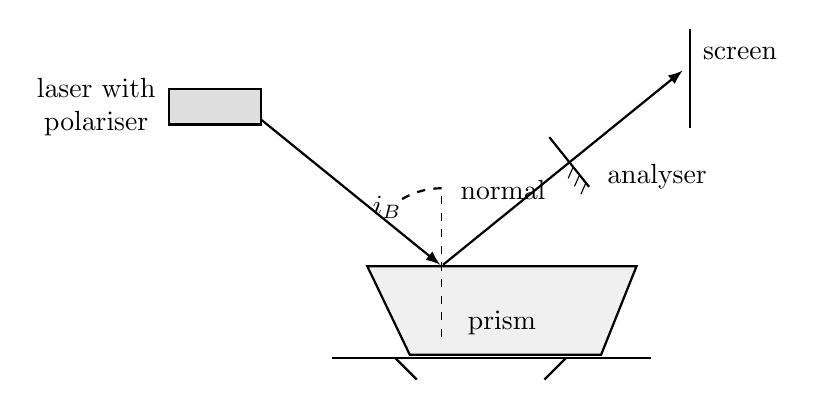
\begin{tikzpicture}[x=0.9cm,y=0.9cm,>=latex]
% platform
\draw[thick] (1.6,0.25) -- (6.1,0.25);
\draw[thick] (2.5,0.25) -- (2.8,-0.05);
\draw[thick] (4.9,0.25) -- (4.6,-0.05);
% prism (glass block with a flat upper face)
\draw[thick,fill=gray!12] (2.1,1.55) -- (5.9,1.55) -- (5.4,0.3) -- (2.7,0.3) -- cycle;
\node at (4.0,0.75) {prism};
% incidence point and normal
\coordinate (P) at (3.15,1.55);
\draw[dashed] (3.15,0.55) -- (3.15,2.55);
\node[right] at (3.28,2.62) {normal};
% incident beam with polariser
\draw[thick,fill=gray!25] (-0.7,3.55) rectangle (0.6,4.05);
\node[left,align=center] at (-0.75,3.8) {laser with\\polariser};
\draw[->,thick] (0.6,3.62) -- (3.13,1.57);
\draw[thick,dashed] (P) ++(90:1.1) arc (90:123:1.1);
\node at (2.38,2.38) {$i_B$};
% reflected beam
\draw[->,thick] (3.17,1.57) -- (6.55,4.31);
% analyser
\draw[thick] (5.23,2.67) -- (4.67,3.37);
\foreach \t in {0.08,0.24,0.40} \draw (5.23-0.56*\t,2.67+0.70*\t) -- (5.16-0.56*\t,2.51+0.70*\t);
\node[right] at (5.35,2.82) {analyser};
% screen
\draw[thick] (6.65,3.5) -- (6.65,4.9);
\node[right] at (6.7,4.55) {screen};
\end{tikzpicture}
\end{figbox}
